\section{Introduktion}
Projektet er skabt for at tilfredstille de nye behov, som \textit{Katrines Kælder} har ønsket gennem en henvendelse til gruppen. \textit{Katrines Kælder} har ønsket et elektronisk kassesystem, som kan føre journal over det salg, som har været i løbet af en åbningsdag. Kassesystemet skal ligeledes kunnne integrere betalinger fra \textit{Dankort}-terminalen.

\subsection{Formål og omfang}
Formålet med dokumentet er at beskrive arkitekturen bag systemet. Arkitekturen er bygget ud fra de krav, som er stillet i kravspecifikationen. Dokumentet vil beskrive designet af systemet uden at gå i dybden i forhold til implementeringen.

\subsection{Referencer}
Referencer vil kunne findes bagerst i dokumentet i afsnittet.

\subsection{Dokumentstruktur og læsevejledning}
Dokumentstrukturen er bygget op omkring N\plus1 modellen, som er en udvidelse af 4\plus1 modellen. Modellen skaber en beskrivelse af systemet ud fra forskellige synspunkter. Dvs. at de forskellige views behandler arkitekturbeskrivelsen anderledes alt efter hvilket view, der er i fokus. Modsat 4\plus1 modellen, som kan ses i figur~\ref{fig:4plus1}, kan N\plus1 indeholde alle de views, som der nødvendige for at skrive en komplet dokumentation af systemet.

\begin{figure}[H]
	\centering
	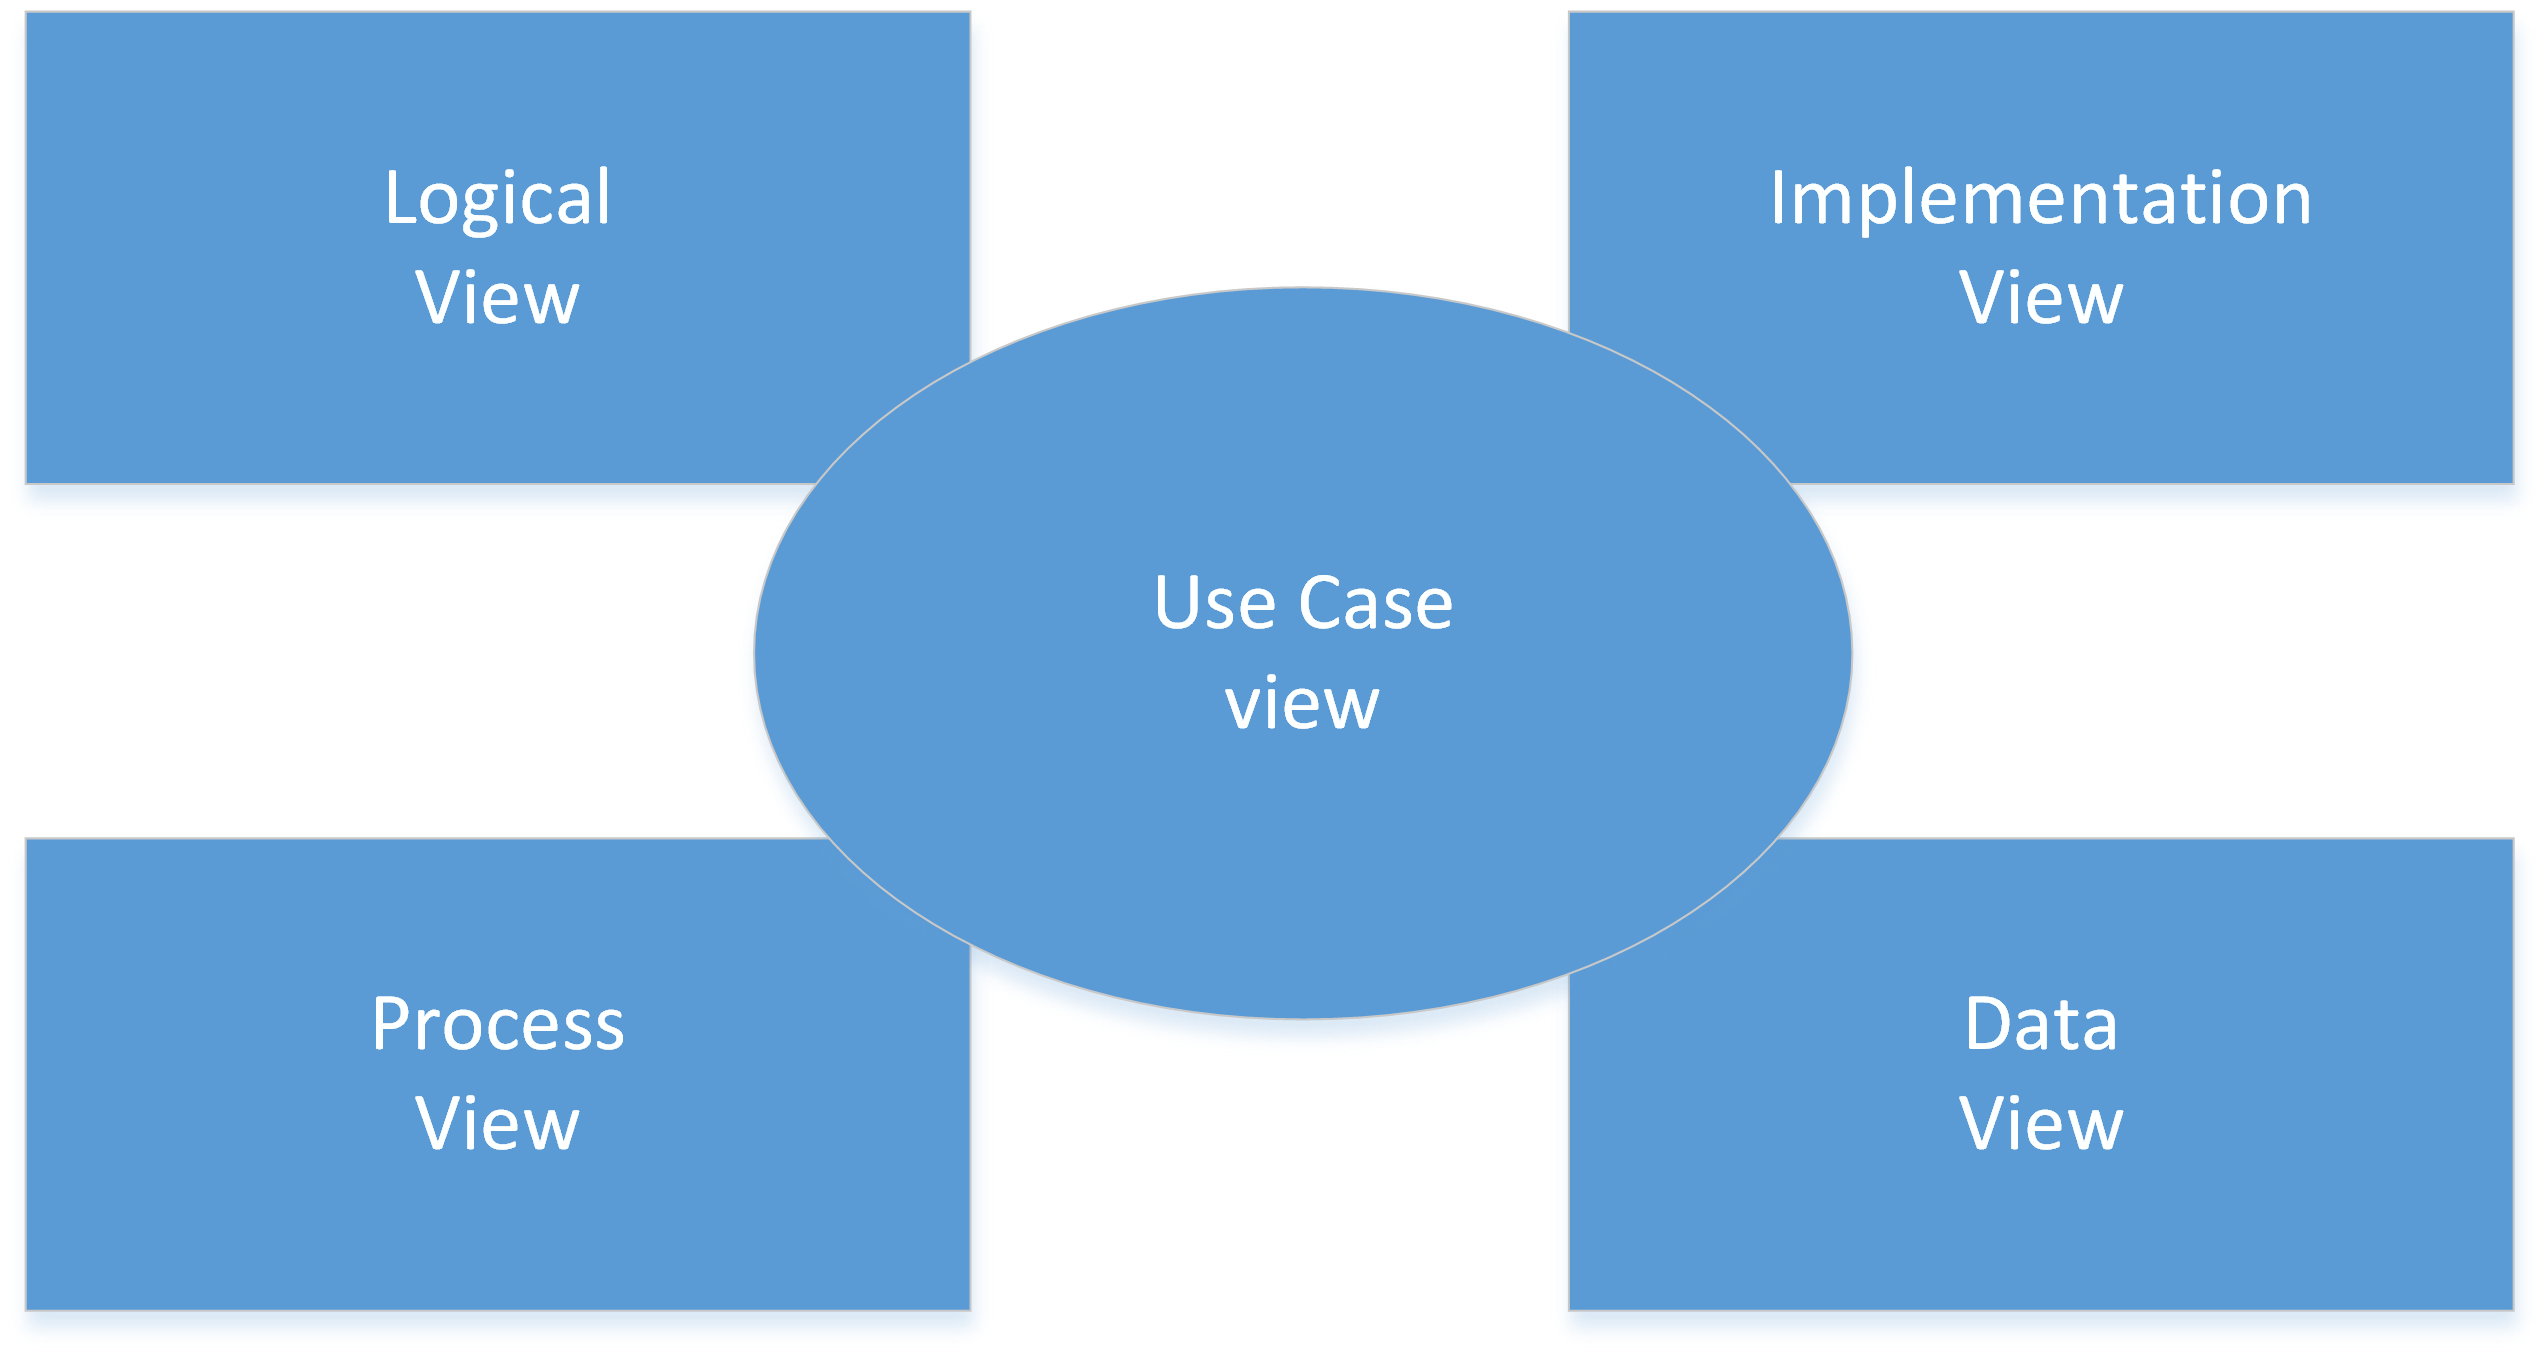
\includegraphics[width=0.7\textwidth]{N+1/Intro/Nplus1.png}
	\caption{4 plus 1 modellen}
	\label{fig:4plus1}
\end{figure}

I dette dokument har vi valgt at indkludere følgende views:

\begin{itemize}
	\item Domain View
	\item Use Case View
	\item Logical View
	\item Process View
	\item Implementation View
	\item Data View
\end{itemize}

\subsubsection{Læsevejledning}
Dokumentet læses fortløbende for at opnå en fuld forståelse af systemet. Enkelte afsnit har referencer tilbage til kravspecifikationen, der skal ses som fundamentet for arkitekturdokumentationen.

\subsection{Dokumentets rolle i en iterativ udviklingsproces}
Dokumentet er en opsamling på det iterative projektarbejde. 
Det er tænkt at dokumentet opdateres løbende med nye use cases og nye realiseringer af disse. 
Det gør at dokumentet virker som en vejledning hvorfra systemet kan implementeres. 
Når der arbejdes iterativt giver det rigtigt god mening at have et dokument der fastsætter hvilke aftaler der er lavet for nuværende sprint.